%%
%% This is file `sample-sigconf.tex',
%% generated with the docstrip utility.
%%
%% The original source files were:
%%
%% samples.dtx  (with options: `all,proceedings,bibtex,sigconf')
%%
%% IMPORTANT NOTICE:
%%
%% For the copyright see the source file.
%%
%% Any modified versions of this file must be renamed
%% with new filenames distinct from sample-sigconf.tex.
%%
%% For distribution of the original source see the terms
%% for copying and modification in the file samples.dtx.
%%
%% This generated file may be distributed as long as the
%% original source files, as listed above, are part of the
%% same distribution. (The sources need not necessarily be
%% in the same archive or directory.)
%%
%%
%% Commands for TeXCount
%TC:macro \cite [option:text,text]
%TC:macro \citep [option:text,text]
%TC:macro \citet [option:text,text]
%TC:envir table 0 1
%TC:envir table* 0 1
%TC:envir tabular [ignore] word
%TC:envir displaymath 0 word
%TC:envir math 0 word
%TC:envir comment 0 0
%%
%%
%% The first command in your LaTeX source must be the \documentclass
%% command.
%%
%% For submission and review of your manuscript please change the
%% command to \documentclass[manuscript, screen, review]{acmart}.
%%
%% When submitting camera ready or to TAPS, please change the command
%% to \documentclass[sigconf]{acmart} or whichever template is required
%% for your publication.
%%
%%
\documentclass[sigconf, hyperref={colorlinks=true,linkcolor=blue,urlcolor=blue}]{acmart}

%%
%% \BibTeX command to typeset BibTeX logo in the docs
\AtBeginDocument{%
  \providecommand\BibTeX{{%
    Bib\TeX}}}

%% Rights management information.  This information is sent to you
%% when you complete the rights form.  These commands have SAMPLE
%% values in them; it is your responsibility as an author to replace
%% the commands and values with those provided to you when you
%% complete the rights form.

% Is this necessary for us?
\setcopyright{acmlicensed}
\copyrightyear{2024}
\acmYear{2024}
\acmDOI{XXXXXXX.XXXXXXX}

%% These commands are for a PROCEEDINGS abstract or paper.
% \acmConference[Conference acronym 'XX]{Make sure to enter the correct
%   conference title from your rights confirmation emai}{June 03--05,
%   2018}{Woodstock, NY}
%%
%%  Uncomment \acmBooktitle if the title of the proceedings is different
%%  from ``Proceedings of ...''!
%%
%%\acmBooktitle{Woodstock '18: ACM Symposium on Neural Gaze Detection,
%%  June 03--05, 2018, Woodstock, NY}
% \acmISBN{978-1-4503-XXXX-X/18/06}


%%
%% Submission ID.
%% Use this when submitting an article to a sponsored event. You'll
%% receive a unique submission ID from the organizers
%% of the event, and this ID should be used as the parameter to this command.
%%\acmSubmissionID{123-A56-BU3}

%%
%% For managing citations, it is recommended to use bibliography
%% files in BibTeX format.
%%
%% You can then either use BibTeX with the ACM-Reference-Format style,
%% or BibLaTeX with the acmnumeric or acmauthoryear sytles, that include
%% support for advanced citation of software artefact from the
%% biblatex-software package, also separately available on CTAN.
%%
%% Look at the sample-*-biblatex.tex files for templates showcasing
%% the biblatex styles.
%%

%%
%% The majority of ACM publications use numbered citations and
%% references.  The command \citestyle{authoryear} switches to the
%% "author year" style.
%%
%% If you are preparing content for an event
%% sponsored by ACM SIGGRAPH, you must use the "author year" style of
%% citations and references.
%% Uncommenting
%% the next command will enable that style.
%%\citestyle{acmauthoryear}


%%
%% end of the preamble, start of the body of the document source.
\begin{document}

%%
%% The "title" command has an optional parameter,
%% allowing the author to define a "short title" to be used in page headers.
\title{Predictors of NFL tackles}

%%
%% The "author" command and its associated commands are used to define
%% the authors and their affiliations.
%% Of note is the shared affiliation of the first two authors, and the
%% "authornote" and "authornotemark" commands
%% used to denote shared contribution to the research.
\author{Isaac Kou (4502)}
\email{Isaac.Kou@colorado.edu}
\affiliation{%
  \institution{University of Colorado Boulder}
  \city{Boulder}
  \state{Colorado}
  \country{USA}
}

\author{Sean Shi (4502)}
\email{Sean.Shi@colorado.edu}
\affiliation{%
  \institution{University of Colorado Boulder}
  \city{Boulder}
  \state{Colorado}
  \country{USA}
}

\author{Timur Tripp (5502)}
\email{Timur.Tripp@colorado.edu}
\affiliation{%
  \institution{University of Colorado Boulder}
  \city{Boulder}
  \state{Colorado}
  \country{USA}
}

\author{Grace Williams (5502)}
\email{Grace.Williams@colorado.edu}
\affiliation{%
  \institution{University of Colorado Boulder}
  \city{Boulder}
  \state{Colorado}
  \country{USA}
}

% \authornote{Both authors contributed equally to this research.}
% \orcid{1234-5678-9012}
% \author{G.K.M. Tobin}
% \authornotemark[1]
% \affiliation{%
%   \institution{Institute for Clarity in Documentation}
%   \city{Dublin}
%   \state{Ohio}
%   \country{USA}
% }

%%
%% By default, the full list of authors will be used in the page
%% headers. Often, this list is too long, and will overlap
%% other information printed in the page headers. This command allows
%% the author to define a more concise list
%% of authors' names for this purpose.
\renewcommand{\shortauthors}{Isaac et al.}

%%
%% The abstract is a short summary of the work to be presented in the
%% article.

%%
%% The code below is generated by the tool at http://dl.acm.org/ccs.cfm.
%% Please copy and paste the code instead of the example below.
%%

%%
%% Keywords. The author(s) should pick words that accurately describe
%% the work being presented. Separate the keywords with commas.
\keywords{Football, Data Mining, CSCI4502, Tackles}
%% A "teaser" image appears between the author and affiliation
%% information and the body of the document, and typically spans the
%% page.

\begin{teaserfigure}
% Random image of tackling I pulled from the internet, feel free to replace
  % \caption{Seattle Mariners at Spring Training, 2010.}
  % \Description{Enjoying the baseball game from the third-base
  % seats. Ichiro Suzuki preparing to bat.}
  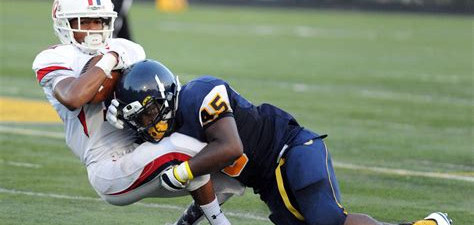
\includegraphics[width=\textwidth]{./th-4169371817}
  \label{fig:teaser}
\end{teaserfigure}

\received{27 September 2024}
% \received[revised]{12 March 2009}
% \received[accepted]{5 June 2009}

%%
%% This command processes the author and affiliation and title
%% information and builds the first part of the formatted document.
\maketitle

\section{Introduction}
What? NFL Big Data Bowl 2024 provided by Next Gen Stats (2022 season data)

Main goal: Predicting tackle time, probability, and location
Provided with player-level tackle information for each weeks games and
plays, as well as position on the field, speed, acceleration, etc.

Why?
Provide NFL with understanding of tackle expectations and limitations in order
to better protect players from injury and improve gameplay

\section{Existing Work}
A significant number of previous academic studies exist on the topic of
tackling in American football. This section discusses three examples of those
studies, one hobbyist analysis, and the foundation they lay for our proposed
work.

The paper \href{https://link.springer.com/article/10.1007/s10439-020-02625-7}{“Validating Tackle
Mechanics in American Football: Improving Safety and Performance”} (Maerlender et al.) discusses the
development of a program to reduce the risk of serious injury from tackling, specifically by identifying
head-contact likelihoods and therefore alternative techniques to reduce such contact. Secondary research
related to the impact of tackles on player performance was also conducted, finding a reduction in
their number of yards run post-contact.

Similarly, \href{https://www.jstage.jst.go.jp/article/ijshs/16/0/16_201804/_article/-char/ja/}
{“Effectiveness of the Heads Up Tackling (HUT) Program on Tackling Safety and Performance in American Football”}
(Matsuo et al.) also identifies a program to promote tackle safety, though this study focuses
on an existing program and its observed impacts. Results indicated that implementation of the
studied HUT Program reduced rate and severity of player injury, with no detriment, or, in some
cases, even benefit, to player performance.

Lastly, \href{https://bmjopensem.bmj.com/content/6/1/e000638.abstract}{“Quantitative and qualitative
analysis of head and body impacts in American 7v7 non-tackle football”} (Jadischke et al.) used video
analysis to investigate the rate of head contact in the alternative non-tackle play style of
American football. In a similar vein to the above studies, this research found that non-tackle
football was associated with lower rates of head contact and therefore potentially lower rates of
injury, though further research is needed.

Outside of academia, many football fans conduct hobbyist analyses of their own, often
concerning points, player performance, game trends, and so on. An example of this is
the article \href{https://medium.com/@ezra.ford/tackling-metrics-with-big-data-0812b5ab65f0}{“Tackling Metrics with Big Data”}
by Ezra Ford on Medium. In addition to being a subject of interest in and of themselves,
these have applications in related sub-hobbies, such as sports betting and fantasy football,
and can help fans maximize their success in those activities.

As shown, the existing work on tackles in American football often concerns the implications of
tackling, instead of the ability to predict and understand when/where/how tackles happen.
Thus, our work intends to investigate these trends instead.

\section{Proposed Work}

To analyze the effect of various traits of player, matches, and other factors on
the timing and a success rate of tackle, we will be using data from the Kaggle
NFL Big Data Bowl
\href{https://www.kaggle.com/competitions/nfl-big-data-bowl-2024/data}{\underline{dataset}}
specifically the files ``\verb|tackles.csv|'', ``\verb|games.csv|'',
``\verb|plays.csv|'' which contain data on the play, players, success, teams,
etc. involved in a tackle.

Our primary goal for this project is to find correlations between previously
known information such as weight, height, and time during a game and the tackles
performed (location, likelihood of success and number of tackles). To this end,
we are proposing to try and find correlations between factors such as height and
weight and frequency and likelihood of success of tackles, frequency analysis
for examining which teams/players tend to engage in tackles, and time series
analysis to understand the relationship between time during a game an frequency
of tackles.

In addition to this analysis, we also seek to analyze whether the risk of injury
from tackles can be reduced and how much of an impact tackles have on the
outcome of a game or visa versa. We will also seek to analyze the difference in
frequencies of tackles between different teams and positions.

\section{Evaluation}
\begin{itemize}
    \item As with any data analysis:
      \begin{itemize}
      \item Want to find enough evidence to disprove the null hypothesis (i.e.,
        disprove that there is no statistical difference between tackle rate that can be
        attributed to X variable, and that any difference seen is due to chance)
      \item
        Cannot necessarily prove hypothesis, but can present findings if null hypothesis is false
      \end{itemize}
    \item Will evaluate our success based on:
      \begin{itemize}
      \item Thoroughness of work and consideration of all factors
      \item Not necessarily finding an “answer”, as one may not exist with real-world data
      \end{itemize}
\end{itemize}

\section{Milestones}
\begin{table}[H]
  \caption{Milestones for the semester}
  \label{tab:freq}
  \begin{tabular}{c|l}
    \toprule
    Date&Milestone\\
    \midrule
     9/24 - 9/26 & Project Proposal (Now) \\
     9/29 - 9/31 & Data cleaning complete \\
                 & Begin initial analysis \\
     11/5 - 11/7 & Project Checkpoint Report \\
   11/12 - 11/14 & Analysis Complete \\
     12/3 - 12/5 & Visualizations in final deliverable form \\
                 & summarize findings   \\
   12/10 - 12/12 & Project Final Report  \\
  \bottomrule
\end{tabular}
\end{table}

\end{document}
\endinput
